\begin{surferPage}[Лабс]{Септика с 99 сингулярностями}
Оливер Лабс сконструировал в ходе работы над своей диссертацией в г. Майнце в 2004 г. поверхность $7$ степени (септику) с $99$ сингулярностями: на сегодняшний день это – мировой рекорд! До настоящего времени не известны причины, которые бы препятствовали наличию септики и со $104$ сингулярностями. 

Поверхность Лабса обладает симметрией правильного семиугольника. Это прекрасно видно, если посмотреть на поверхность «сверху». 
    \vspace*{-0.3em}
    \begin{center}
      \begin{tabular}{c@{\qquad}c}
        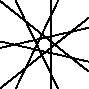
\includegraphics[height=1.5cm]{./../../common/images/labsseptic1.pdf}
        &
        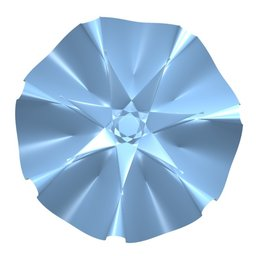
\includegraphics[height=1.5cm]{./../../common/images/labs_septic_von_oben}
      \end{tabular}
    \end{center}
    \vspace*{-0.3em}

Для поиска поверхности О. Лабс использовал компьютерную программу Singular (Университет г. Казерслаутерна), сильные стороны которой заключаются в её приложении в сфере алгебраической геометрии и сингулярностей.

При этом он пользовался тем, что можно вести расчёты в конечных числовых системах. Это похоже на то, как мы считываем время с часов: $24\,$ч. соответствуют $0\,$ч., $24\,\text{ч}. + 1\,$ч. – не $25\,$ч., а $1\,$ч.
\end{surferPage}
